\def\chaptername{Κεφάλαιο}
\chapter{Εισαγωγή}
\def\chaptername{Chapter}

\section{Κίνητρο}

Στη σύγχρονη εποχή, τα δεδομένα κοινωνικής δικτύωσης, τα οποία παράγονται και  
διαχειρίζονται καθημερινά από τις αντίστοιχες υπηρεσίες, αυξάνονται με ραγδαίους ρυθμούς. 
Επιπλέον, τα δεδομένα αυτά περιέχουν πληροφορίες κείμενου, φωτογραφίας, βίντεο, χρόνου και τοποθεσίας. Ενδεικτικά, η διαδικτυακή υπηρεσία κοινωνικής δικτύωσης Twitter, 
σύμφωνα με τα επίσημα στατιστικά \cite{1}, διαθέτει 302 εκατομμύρια ενεργούς χρήστες κάθε μήνα και διαχειρίζεται κάθε μέρα 500 εκατομμύρια μηνύματα (tweets) 
τα οποία δημοσιεύονται από τους χρήστες. Τα tweets περιλαμβάνουν στοιχεία κειμένου και χρόνου (η ώρα δημοσίευσης) και μπορεί να περιέχουν επίσης 
εικόνα, βίντεο και \linebreak πληροφορίες τοποθεσίας. Τα παραδοσιακά μέσα αποθήκευσης και τεχνικές επεξεργασίας δεν \linebreak επαρκούν πλέον για τον τεράστιο όγκο των πολύμορφων 
κοινωνικών δεδομένων. Για το λόγο αυτό, οι σύγχρονες υπηρεσίες κοινωνικής δικτύωσης 
καταφεύγουν σε κατανεμημένα συστήματα και εργαλεία διαχείρισης δεδομένων. Για παράδειγμα, η υπηρεσία Twitter αρχικά 
αποθήκευε τα tweets των \linebreak χρηστών σε παραδοσιακές βάσεις δεδομένων \cite{2}. Όμως, με το πέρασμα του καιρού και την τεράστια αύξηση των 
tweets, υπήρχαν προβλήματα στην ανάγνωση και εγγραφή δεδομένων στις βάσεις αυτές. Έτσι, η υπηρεσία δημιούργησε και χρησιμοποίησε κατανεμημένα εργαλεία αποθήκευσης 
για τα \linebreak δεδομένα τα οποία έπρεπε να διαχειριστεί \cite{4}. Με τα εργαλεία αυτά παρατηρήθηκε σημαντική \linebreak βελτίωση στην επίδοση της υπηρεσίας. 

Ένας μεγάλος αριθμός από διαδικτυακές υπηρεσίες χρησιμοποιούν πλέον κατανεμημένα \linebreak συστήματα αποθήκευσης δεδομένων. Για παράδειγμα, μεγάλες διαδικτυακές 
υπηρεσίες, όπως το Twitter και το Yahoo!, χρησιμοποιούν το κατανεμημένο σύστημα βάσης δεδομένων HBase, για τη διαχείριση 
ενός τμήματος των δεδομένων τους \cite{4}. Αντίστοιχα, πολλές διαδικτυακές υπηρεσίες κοινωνικής δικτύωσης, όπως το Facebook και το Twitter, 
χρησιμοποιούν το \linebreak κατανεμημένο σύστημα διαχείρισης δεδομένων Hadoop \cite{6}. Η ελεύθερη γνώση των \linebreak 
συστημάτων τα οποία χρησιμοποιούν οι 
υπηρεσίες αυτές, λόγω του γεγονότος ότι είναι συστήματα ανοιχτού κώδικα, μας δίνει μία πρώτη εικόνα της 
λειτουργίας τους. Όμως, τα δεδομένα τα οποία διαχειρίζονται δε γίνονται διαθέσιμα στο ευρύ κοινό, για λόγους 
διαφύλαξης των προσωπικών \linebreak δεδομένων των χρηστών. Έτσι, δε μπορούμε να κατανοήσουμε πλήρως τη λειτουργία των υπηρεσιών αυτών και να αξιολογήσουμε την επιλογή 
των συγκεκριμένων κατανεμημένων εργαλείων για τη διαχείρηση των δεδομένων τους. 

Με την παρούσα διπλωματική εργασία, ερχόμαστε να καλύψουμε αυτό το κενό στην πλήρη κατανόηση της διαχείρισης δεδομένων χρηστών κατά την λειτουργία των υπηρεσιών κοινωνικής δικτύωσης. 
Εφ'όσον δε μπορούμε να έχουμε πρόσβαση στα αντίστοιχα δεδομένα, προσπαθήσαμε να δημιουργήσουμε ρεαλιστικά 
δεδομένα κοινωνικής δικτύωσης, τα οποία να προσομοιάζουν 
σε μεγάλο βαθμό αντίστοιχα 
πραγματικά δεδομένα. Για το σκοπό αυτό, σχεδιάσαμε και υλοποιήσαμε μία γεννήτρια ρεαλιστικών χωροχρονικών δεδομένων, στα πρότυπα 
αυτών που συναντάμε σε μεγάλες υπηρεσίες κοινωνικής δικτύωσης, όπως το Facebook. 

\newpage

\section{Κύρια σημεία της εργασίας}

Οι βασικές συνεισφορές της διπλωματικής εργασίας είναι οι ακόλουθες:

\begin{enumerate}
 \item Σχεδιασμός και υλοποίηση παραμετροποιήσιμης γεννήτριας χωροχρονικών δεδομένων \linebreak ανοιχτού κώδικα \footnote{Ο κώδικας είναι διαθέσιμος στο 
 \url{https://github.com/Thaleia-DimitraDoudali/thesis}}.
 \item Δημιουργία συνόλου χωροχρονικών δεδομένων μεγάλου όγκου με χρήση της γεννήτριας.
 \item Αποδοτική αποθήκευση και δεικτοδότηση του συνόλου δεδομένων σε κατανεμημένο σύστημα διαχείρισης δεδομένων.
 \item Πειραματική αξιολόγηση της κλιμακωσιμότητας του συστήματος διαχείρισης δεδομένων, κάτω από διαφορετικό όγκο δεδομένων, ταυτόχρονα 
 συνδεδεμένων χρηστών και αριθμών κόμβων.
\end{enumerate}

\section{Οργάνωση κειμένου}

Στη συνέχεια του κεφαλαίου 1 ακολουθεί μία σύντομη περιγραφή του σχεδιασμού της γεννήτριας χωροχρονικών δεδομένων. Επίσης, αναφέρονται συνοπτικά τα 
αποτελέσματα της αποτιμήσης των υπηρεσιών κοινωνικής δικτύωσης μέσω της υλοποίησης και εφαρμογής επερωτήσεων στο σύνολο δεδομένων μεγάλου όγκου, 
τα οποία δημιουργήθηκαν από την γεννήτρια και αποθηκεύτηκαν σε ένα συτημα κατανεμημένης διαχείρισης δεδομένων.

Στο κεφάλαιο 2 παρουσιάζεται το θεωρητικό υπόβαθρο, το οποίο είναι σημαντικό να γνωρίζει κάποιος, ώστε να κατανοήσει έννοιες και ορολογίες που θα αναφέρονται 
στη συνέχεια. Ενδεικτικά, αναλύονται τα εργαλεία που χρησιμοποιήθηκαν στην υλοποίηση της γεννήτριας, όπως η βάση \linebreak δεδομένων για τα πηγαία δεδομένα, 
οι υπηρεσίες της Google για τη δημιουργία και παρουσίαση των τροχιών και ορισμένες μαθηματικές έννοιες για τις παραμέτρους εισόδου. Επίσης, 
παρουσιάζονται τα κατανεμημένα εργαλεία αποθήκευσης και διαχείρισης δεδομένων, τα οποία χρησιμοποιήθηκαν για τα παραγόμενα από τη γεννήτρια δεδομένα. 

Στο κεφάλαιο 3 παρατίθεται μία λεπτομερής περιγραφή της μεθοδολογίας σχεδιασμού της \linebreak γεννήτριας χωροχρονικών δεδομένων. Αναλύεται ο τρόπος αποθήκευσης των πηγαίων 
δεδομένων, ορίζονται οι παράμετροι εισόδου της γεννήτριας και περιγράφονται με λεπτομέρεια οι οντότητες, οι αποφάσεις, οι παραδοχές και η πλήρης λειτουργία της 
γεννήτριας. 

Στο κεφάλαιο 4 αναλύεται ο τρόπος δημιουργίας ενός συνόλου δεδομένων μεγάλου όγκου \linebreak παραγόμενων από τη γεννήτρια, καθώς και το σχήμα δεδομένων για την αποθήκευσή του 
σε μία κατανεμημένη βάση δεδομένων. 

Στο κεφάλαιο 5 παρατίθεται η μεθοδολογία υλοποίησης των επερωτήσεων στο σύνολο των \linebreak διαθέσιμων δεδομένων τα οποία παράχθηκαν από τη γεννήτρια. Επίσης, 
παρουσιάζονται τα \linebreak αποτελέσματα από την αξιολόγηση της κλιμακωσιμότητας του συστήματος της βάσης δεδομένων στην οποία αποθηκεύτηκαν τα δεδομένα μέσω 
της εκτέλεσης των επερωτήσεων αυτών στα δεδομένα. 

Στο κεφάλαιο 6 ανακεφαλαιώνονται τα συμπεράσματα της παραπάνω αποτίμησης των εργαλείων αποθήκευσης και επεξεργασίας δεδομένων που χρησιμοποιούν 
οι υπηρεσίες κοινωνικής δικτύωσης. Επίσης, παρουσιάζονται σχετικές εργασίες και πιθανές 
μελλοντικές επεκτάσεις της τρέχουσας \linebreak διπλωματικής. 


\section{Συνοπτική περιγραφή της γεννήτριας}

Η θεμελιώδης λειτουργία της γεννήτριας είναι η παραγωγή ρεαλιστικών χωροχρονικών \linebreak δεδομένων. 
Πιο συγκεκριμένα, η γεννήτρια δημιουργεί χρήστες υπηρεσιών κοινωνικής δικτύωσης, οι οποίοι κάθε μέρα επισκέπτονται διάφορα 
σημεία ενδιαφέροντος για τα οποία αφήνουν μία κριτική και βαθμολογία στην πλατφόρμα. Επομένως, η γεννήτρια παράγει ημερήσιες τροχιές χρηστών για ένα 
καθορισμένο χρονικό διάστημα. 

Η γεννήτρια ρεαλιστικών χωροχρονικών δεδομένων χρησιμοποιεί πραγματικά σημεία \linebreak ενδιαφέροντος ως πηγή δεδομένων. Τα σημεία αυτά προμηθεύτηκαν από την υπηρεσία 
ταξιδιών κοινωνικής δικτύωσης TripAdvisor. Τα πηγαία δεδομένα περιέχουν τις γεωγραφικές συντεταγμένες, την ονομασία και διεύθυνση των σημείων ενδιαφέροντος, 
καθώς και μία λίστα από κριτικές και βαθμολογίες για τα αντίστοιχα σημεία από πραγματικούς χρήστες της υπηρεσίας. Για την αποθήκευση των δεδομένων αυτών 
χρησιμοποιήθηκε η βάση δεδομένων PostgreSQL, έτσι ώστε να έχουμε \linebreak πρόσβαση στις συναρτήσεις χειρισμού γεωγραφικών τύπων δεδομένων και 
υπολογισμού αποστάσεων μεταξύ γεωγραφικών σημείων, οι οποίες παρέχονται 
από την επέκταση PostGIS την οποία διαθέτει η PostgreSQL. Η γεννήτρια λαμβάνει ορισμένες παραμέτρους εισόδου, έτσι ώστε να παραμετροποιείται η λειτουργία της 
και να τροποποιείται το πλήθος και εν μέρει η δομή των παραγόμενων δεδομένων. Ενδεικτικά, οι παράμετροι αφορούν το πλήθος των χρηστών που θα παραχθούν, το 
χρονικό διάστημα για το οποίο θα δημιουργθούν ημερήσιες τροχιές για όλους τους χρήστες και ορισμένες μετρικές που επηρεάζουν τις ημερήσιες επισκέψεις των χρηστών 
στα σημεία ενδιαφέροντος.

Η γεννήτρια κατά τη δημιουργία των ημερήσιων τροχιών λαμβάνει αποφάσεις οι οποίες βασίζονται σε παράγοντες τυχαιότητας. Πιο συγκεκριμένα, τα σημεία 
ενδιαφέροντος τα οποία επισκέπτεται κάθε χρήστης καθορίζονται με τυχαίο τρόπο από τη γεννήτρια, με μόνο περιορισμό να είναι σε κοντινή απόσταση μεταξύ τους και από 
την κατοικία του χρήστη. Η κατοικία κάθε χρήστη ορίζεται και αυτή με τυχαίο τρόπο και η σχετική απόσταση καθορίζεται από παράμετρο εισόδου. Οι χρήστες έχουν 
τη δυνατότητα να πραγματοποιούν ταξίδια, έτσι ώστε να επισκέπτονται και σημεία ενδιαφέροντος σε πιο μακρινή απόσταση. Η τοποθεσία και διάρκεια του ταξιδιού 
καθορίζονται και αυτές με τυχαίο τρόπο. Η γεννήτρια επιτρέπει σε ένα χρήστη να επισκέπτεται κάποιο σημείο μόνο μία φορά την ημέρα. Σε κάθε σημείο στο οποίο 
ο χρήστης κάνει check-in, η γεννήτρια αναθέτει μία τυχαία κριτική και βαθμολογία για το σημείο αυτό από το συγκεκριμένο χρήστη. Η κριτική αυτή και η βαθμολογία 
του σημείου αυτού είναι πραγματική, όπως την έγραψε κάποιος χρήστης της υπηρεσίας TripAdvisor.

Σχετικά με τη διαδρομή από ένα σημείο 
ενδιαφέροντος στο επόμενο, ο χρήστης περπατά για να μεταβεί στον προορισμό του, γι'αυτό και η απόσταση μεταξύ των σημείων έχει νόημα να είναι κοντινή και 
καθορίζεται από αντίστοιχη παράμετρο εισόδου. Η γεννήτρια χρησιμοποιεί την υπηρεσία εύρεσης διαδρομών της Google (Google Directions API) \cite{16}. 
Στέλνει μία αίτηση στην υπηρεσία, 
η οποία τελικά επιστρέφει ένα αρχείο απάντησης με αναλυτικές οδηγίες και πληροφορίες για τη διαδρομή. Από το αρχείο αυτό η γεννήτρια αξιοποιεί το σύνολο των σημείων της 
διαδρομής, τα οποία επιστρέφει η υπηρεσία, ως στίγματα δορυφόρου που υποδεικνύουν τη διαδρομή. Η γεννήτρια λαμβάνει, επίσης, από το αρχείο απάντησης και τη διάρκεια 
της διαδρομής από το σημείο αρχής στο σημείο προορισμού. Με την πληροφορία αυτή, μπορεί να υπολογίσει και τη χρονική στιγμή την οποία ο χρήστης θα κάνει check-in στο 
επόμενο σημείο. Το πλήθος των σημείων ενδιαφέροντος τα οποία θα επισκεφτεί ο χρήστης κατά τη διάρκεια της ημέρας καθορίζονται με τυχαίο τρόπο, όπως και 
η διάρκεια της επίσκεψης σε κάθε σημείο. Τέλος, η γεννήτρια χρησιμοποιεί την υπηρεσία στατικού χάρτη της Google (Google Static Maps API) \cite{18}, προκειμένου να 
απεικονίσει στο χάρτη τις ημερήσιες διαδρομές των χρηστών. 

Συμπερασματικά, τα δεδομένα τα οποία παράγει η γεννήτρια προσομοιάζουν σε μεγάλο βαθμό πραγματικά δεδομένα κοινωνικής δικτύωσης. Αυτό οφείλεται 
στη χρήση πραγματικών σημείων ενδιαφέροντος ως πηγαία δεδομένα, πραγματικών κριτικών που αναφέρονται στα δεδομένα αυτά, ρεαλιστικών τροχιών
και διαρκειών όπως αυτές παράγονται από το Google Directions API, καθώς   
και στην αξιοποίηση παραγόντων τυχαιότητας στις αποφάσεις τις οποίες λαμβάνει η γεννήτρια. 


\section{Σύνοψη πειραματικής αξιολόγησης}

Η γεννήτρια εκτελέστηκε για ένα σημαντικό χρονικό διάστημα με σκοπό τη δημιουργία ενός συνόλου χωροχρονικών δεδομένων και δεδομένων κειμένου μεγάλου όγκου. 
Πιο συγκεκριμένα, δημιουργήθηκαν 9464 χρήστες, 1586537 επισκέψεις χρηστών και 38800019 δορυφορικά στίγματα, τα οποία αντιστοιχούν σε συνολικά δεδομένα μεγέθους 3 GB. 
Στα δεδομένα αυτά, προσθέσαμε και έναν γράφο φίλων της υπηρεσίας κοινωνικής δικτύωσης Twitter τον οποίο είχαμε στη διάθεσή μας. 
Τα δεδομένα αυτά αποθηκεύτηκαν με ένα συγκεκριμένο σχήμα στην κατανεμημένη βάση. 

Στη συνέχεια, 
υλοποιήθηκαν συγκεκριμένες επερωτήσεις στα δεδομένα αυτά με εργαλεία που αξιοποιούν αποδοτικά όλους τους κόμβους του κατανεμημένου συστήματος. 
Πιο συγκεκριμένα, οι επερωτήσεις αυτές είναι οι ακόλουθες: 
\begin{enumerate}
 \item Για ένα τυχαίο χρήστη της υπηρεσίας, βρες το σημείο ενδιαφέροντος το οποίο επισκέφτηκε τις περισσότερες φορες.
 \item Για ένα τυχαίο χρήστη της υπηρεσίας, εμφάνισε κατα χρονολογική σειρά τις επισκέψεις όλων των φίλων του για μία συγκεκριμένη ημέρα.
 \item Για ένα τυχαίο χρήστη της υπηρεσίας, βρες ποιοι φίλοι του και πόσες φορές έχουν επισκεφτεί το σημείο το οποίο ο ίδιος έχει επισκεφτεί τις περισσότερες φορές. 
\end{enumerate}

Εκτελέσαμε τις επερωτήσεις αυτές με ταυτόχρονο ρυθμό για μεταβλητό συνολικό πλήθος \linebreak επερωτήσεων. Επίσης, μεταβάλλαμε τον αριθμό κόμβων της κατανεμημένης βάσης 
δεδομένων και με τον τρόπο αυτό αξιολογήσαμε την κλιμακωσιμότητα του συστήματος βάσης. Τα αποτελέσματα της εκτέλεσης αυτής συνοψίζονται στα ακόλουθα 
διαγράμματα:

\begin{figure}[H]
    \centering
    \begin{subfigure}[t]{0.5\textwidth}
        \centering
        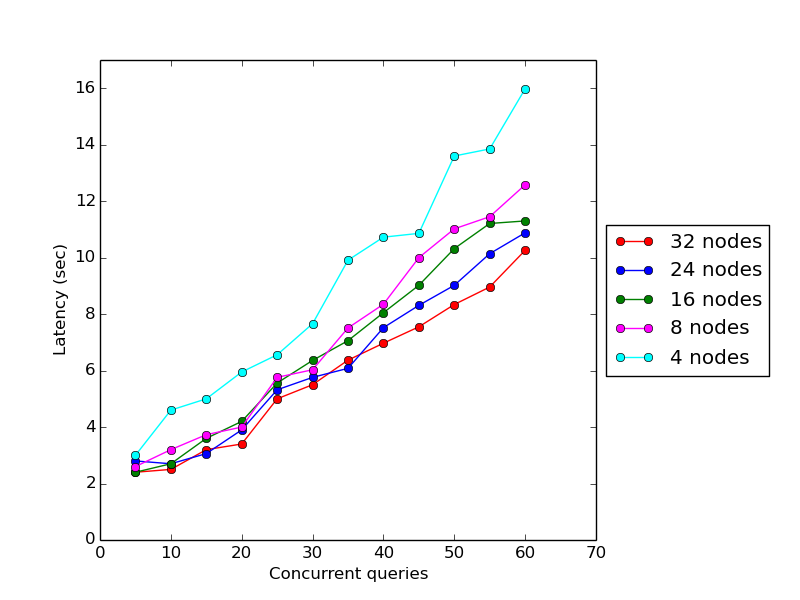
\includegraphics[height=2.4in]{figures/scalability_latency.png}
        \caption{Μέσος χρόνος εκτέλεσης επερωτήσεων}
    \end{subfigure}%
    ~ 
    \begin{subfigure}[t]{0.5\textwidth}
        \centering
        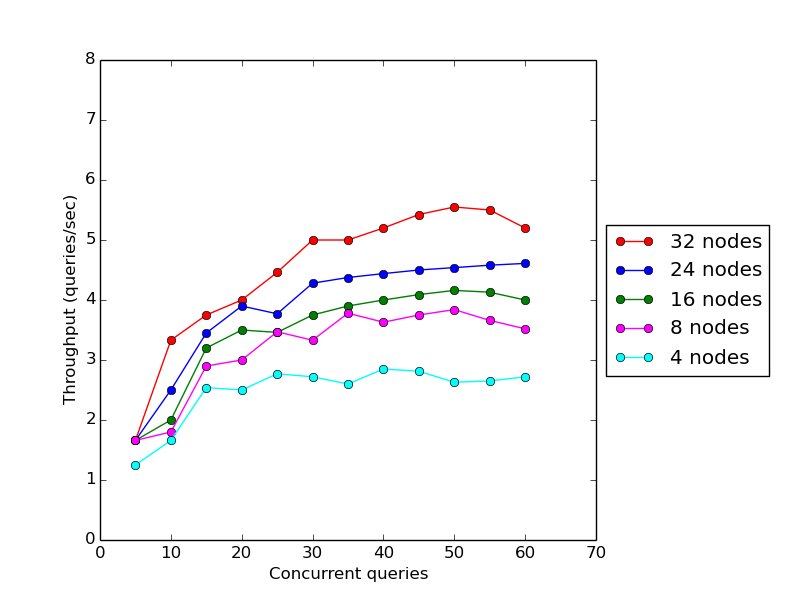
\includegraphics[height=2.4in]{figures/scalability_throughput.png}
        \caption{Ρυθμαπόδοση}
    \end{subfigure}
    \caption{Μετρήσεις κλιμακωσιμότητας}
\end{figure}

Από τα παραπάνω διαγράμματα παρατηρούμε ότι ο μέσος χρόνος εκτέλεσης των επερωτήσεων είναι μεγαλύτερος όσο αυξάνεται το 
πλήθος των ταυτόχρονων επερωτήσεων. Αυτό είναι λογικό από τη στιγμή που οι εξυπηρετητές πρέπει να διαχειριστούν και να διεκπεραιώσουν περισσότερα αιτήματα, οπότε 
κάποια αιτήματα θα περιμένουν στις ουρές των εξυπηρετητών όσο εκείνοι \linebreak διεκπεραιώνουν προηγούμενα αιτήματα. Για το λόγο αυτό, 
παρατηρούμε ότι για διαφορετικό αριθμό κόμβων o μέσος χρόνος εκτέλεσης μικρού πλήθους ταυτόχρονων επερωτήσεων είναι παραπλήσιος, καθώς αυτά απαντούνται 
άμεσα χωρίς να περιμένουν σε ουρές αναμονής. 
Επίσης, ο μέσος χρόνος εκτέλεσης αυξάνεται όσο μειώνεται το πλήθος των κόμβων. Και αυτό είναι αναμενόμενο, καθώς μικρότερο πλήθος κόμβων δε μπορεί να εξυπηρετήσει τα ίδια και 
περισσότερα αιτήματα με τον ίδιο ρυθμό.

Όσον αφορά τη ρυθμαπόδοση του συστήματος, παρατηρούμε ότι αυτή μειώνεται όσο αυξάνεται το πλήθος των κόμβων. Αυτό δικαιολογείται από το γεγονός ότι λιγότεροι κόμβοι 
μπορούν να \linebreak εξυπηρετήσουν τα αιτήματα με πιο αργό ρυθμό καθώς δέχονται περισσότερα ταυτόχρονα αιτήματα από ότι αν υπήρχαν περισσότεροι εξυπηρετητές. Παρ'όλα αυτά βλέπουμε 
ότι υπάρχει μία μέγιστη τιμή στην οποία μπορεί να φτάσει η ρυθμαπόδοση για κάθε πλήθος κόμβων. Αυτό συναντάται σε όλα τα αντίστοιχα πραγματικά συστήματα και δείχνει ότι 
παρ'όλο που υπάρχουν περισσότεροι εξυπηρετητές, υπάρχει ένα άνω όριο στον αριθμό των επερωτήσεων που μπορούν να διεκπεραιώσουν στη μονάδα του χρόνου. Οι 
μικρές διακυμάνσεις στη μέγιστη αυτή τιμή οφείλονται στο γεγονός ότι οι επερωτήσεις αφορούν τυχαίο μέρος των δεδομένων. Επίσης, μπορεί να οφείλονται στο γεγονός ότι 
οι εξυπηρετητές χρησιμοποιούν και κρυφή μνήμη για τα δεδομένα που διαβάζουν από το δίσκο, με την ανάγνωση από την κρυφη μνήμη να είναι πολύ ταχύτερη. Επιπρόσθετα, 
το σύστημα κατανεμημένης μνήμης φιλοξενείται σε εικονικές μηχανές ενός υπολογιστικού νέφους, με αποτέλεσμα η λειτουργία του να επηρεάζεται από τους 
υπόλοιπους ταυτόχρονους χρήστες του νέφους. 

Εν κατακλείδι, συμπεραίνουμε ότι το σύστημα κατανεμημένης μνήμης είναι κλιμακώσιμο για το συγκεκριμένο σχήμα αποθήκευσης των παραγόμενων 
από τη γεννήτρια δεδομένων μεγάλου όγκου, καθώς παρουσιάζει τη χαρακτηριστική συμπεριφορά ενός κλιμακώσιμου συστήματος. 


